\section{A new corpus for natural language inference}\label{sec:discussion}

\todo{Rewrite and expand motivation here (CP?)}

Our ultimate aim in this work is to develop supervised models for sentence representation that can accurately capture natural language meaning. While sentiment tasks like SST have provided a useful testbed for sentence representation models, sentiment labeling only requires that models be able to encode a small piece of the full expressive capacity of language. We claim that the task of natural language inference (also called recognizing textual entailment, or RTE) is significantly more demanding, and that strong performance on this task is good evidence of a model's overall strength in sentence representation.

\subsection{Grounding with imagined images}

\todo{Rewrite and expand (CP?)}

Quote from SICK paper \cite{marelli2014sick}:

\begin{quote}
Not unreasonably, subjects found that, say, \ii{A woman is wearing an Egyptian headdress} does not contradict \ii{A woman is wearing an Indian headdress}, since one could easily imagine both sentences truthfully uttered to refer to a single scene where two different women are wearing different headdresses. In the future, a higher proportion of CONTRADICTION labels could be elicited by using grammatical and possibly visual cues (pictures) encouraging co-indexing of the entities in the two sentences.
\end{quote}

\todo{SICK is referenced below, so we should set it up as a point of reference either here or in the intro, including mentioning that it had both entailment and similarity labels.}

\subsection{Data collection}

We used Amazon Mechanical Turk for data collection. In each individual task (each HIT), a worker was presented with premise scene descriptions from a preexisting corpus, and asked to supply hypotheses that fit each of our three labels (\ii{entailment}, \ii{neutral}, and \ii{contradiction}), forcing the resulting data to be balanced among these classes.

For the premises, we used the Flickr30k corpus \cite{hodoshimage}, a collection of approximately 160k captions from that corpus (corresponding to about 30k images) collected in an earlier crowdsourced effort. The captions were not authored by the photographers who took the source images, they tend to contain relatively literal scene descriptions that are suited to our approach, rather than those typically associated with personal photographs (as in their example: \textit{``Our trip to the Olympic Peninsula''}). We presented each caption to at least one worker, and some to more than one. With the exception of a handful that were flagged by workers as excessively difficult, at least three labeled pairs are available for each caption.

The instructions that we provided to the workers are shown in Fig.~\ref{instructions-1}. Below the instructions were three fields for each of three requested sentences, corresponding to our \ii{entailment}, \ii{neutral}, and \ii{contradiction} labels, a fourth field (marked optional) for reporting problems, and a link to an FAQ page. That FAQ grew over the course of data collection, but discussed disallowed techniques (e.g., reusing the same sentence for many different prompts, which we saw in a few cases), sentence length and complexity (we did not enforce a minimum length, and we allowed bare NPs as well as full sentences), and logistical issues around payment timing. About 2500 workers contributed data.

\begin{figure}
\footnotesize
We will show you the caption for a photo. We will not show you the photo. Using only the caption and what you know about the world:
\begin{itemize}
\item Write one alternate caption that is \textbf{definitely} a \textbf{true} description of the photo. \ii{Example: For the caption "Two dogs are running through a field." you could write "There are animals outdoors."}
\item Write one alternate caption that \textbf{might be} a \textbf{true} description of the photo. \ii{Example: For the caption "Two dogs are running through a field." you could write "There are animals outdoors."}
\item Write one alternate caption that is \textbf{definitely} a \textbf{false} description of the photo. \ii{Example: For the caption "Two dogs are running through a field." you could write "There are animals outdoors." This is different from the maybe correct category because its impossible for the dogs to be both running and sitting.}
\end{itemize}
\todo{Fix the broken examples here (SB)}
\caption{\label{instructions-1}The instructions used on Mechanical Turk for data collection.}
\end{figure}

\subsection{Data validation}

The majority of the sentence pairs in the corpus have not been reviewed by anyone since their construction as part of the data collection Mechanical Turk task, except to remove a small number of responses where either a response field was empty or the original author flagged the source caption for review. In order to measure the quality of our corpus, and in order to construct maximally useful testing and development sets, we did perform an additional round of validation for about 10\% of our data.

This validation phase is not fundamentally different from the Mechanical Turk labeling task used to label the SICK entailment data: we present workers with pairs of sentences (in our case, in batches of five at a time), and ask them to choose a single label for each pair. We supplied each pair to four annonators, yielding five labels per pair including the label used by the original composer of the pair. The instructions were broadly similar to the instructions for initial data collection shown in Fig.~\ref{instructions-1}, and linked to a similar FAQ. Though we used a very restrictive qualification (based on past approval rate) to select workers, we nonetheless discovered and deleted some instances of random guessing during an early round of validation, and subsequently instituted a fully closed qualification restricted to about 30 trusted workers.

For each pair that we validated, we chose a gold label. If any one of the three labels was chosen by at least three of the five annotators, that label is the gold label. If there was no such consensus, which occurred in about 0.2\% of cases, we chose the label `-'. While these unlabeled examples are included in the corpus distribution, they are unlikely to be helpful for the core classification task of NLI, and we do not include them when training and evaluating the models discussed in later sections. The results of this validation process are summarized in Tables \ref{validation-stats} and \ref{validation-freq}, and suggest that while fundamental limits of both our crowdsourcing methods and the task itself impose an upper bound on the consistency of our labels, the data is sufficiently high quality to pose a challenging but realistic machine learning task.



\subsection{The distributed corpus}
\todo{Update all statistics to reflect the latest relase candidate.}


\begin{table*}
  \centering\footnotesize
  \begin{tabular}{p{7.5cm}lp{5.5cm}}
  \toprule
A young man in a striped hoodie looks at an artistic Levi's advertisement that says "We are all workers." & \ii{entailment} & There is a man in a hoodie looking at an advertisement.\\
\rule{0pt}{3ex}Two men on laptops in a dark room. & \ii{entailment} & Two men are on their laptops.\\
\rule{0pt}{3ex}A naked baby and toddler smear each other in paint. & \ii{neutral} & The kids are in the bathtub.\\
\rule{0pt}{3ex}A woman is focusing on her game of curling. & \ii{neutral} & There is a women playing a game indoors\\
\rule{0pt}{3ex}A group of people dressed in green and white are dancing in a circle outside of a white building. & \ii{contradiction} & A group performs indoors.\\
\rule{0pt}{3ex}A balding professor giving a lecture to students on the topic of "opportunity". & \ii{neutral} & A female professor with hair giving a lecture to students.\\
    \bottomrule
% From 1.0rc2
  \end{tabular}
  \caption{\label{snli-examples}Randomly chosen examples from SNLI.\\
\todo{Replace with *validated* examples from the post-rc2 training set, include all 5 labels.}}
\end{table*}

Table~\ref{snli-examples} shows a set of randomly chosen validated examples from the development sent with their labels. Qualitatively, we find the data that we collected to draw fairly extensively on commonsense knowledge, suggesting that superficial word alignment models are unlikely to be able to succeed at classification. We find the sentences that we collected be largely fluent, correctly spelled English, with a mix of full sentences and bare noun phrases of a style that is appropriate for the underlying caption task. Punctution and capitalization are only intermittently present.

The data will be released upon publication under a CreativeCommons
Attribution-ShareAlike licence, the same licence used for the Flickr30k source captions.

\begin{figure}
\center
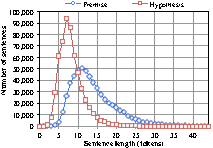
\includegraphics[width=3.05in]{length_dist}
    % From 1.0rc2
\caption{\label{b-table}The distribution of sentence length.} 
\end{figure}

\begin{table}
\center
  %\setlength{\tabcolsep}{15pt}
  %\renewcommand{\arraystretch}{1.2}
  \begin{tabular}{l l} 
    \toprule
Training pairs &  550,153\\
Development pairs &  10,000\\
Test pairs & 10,000\\
\midrule
Premise mean token count & 14.1\\
Hypothesis mean token count & 8.3 \\
\midrule
Premise `S'-rooted parses & 74.0\%\\
Hypothesis `S'-rooted parses & 88.9\%\\
    \bottomrule
  \end{tabular}
% From 1.0rc3
\caption{\label{collection-stats}Key statistics for the raw sentence pairs. Since the two halves of each pair were collected separately, we report statistics for both.} 
\end{table}

\begin{table}
\center
  %\setlength{\tabcolsep}{15pt}
  %\renewcommand{\arraystretch}{1.2}
  \begin{tabular}{l l} 
    \toprule
Validated pairs & 59,445\\
gold label $\ne$ original label & 8.4\%\\
Unanimous gold & 58.2\%\\
No gold (no 3 labels match) & 1.9\%\\
Label $=$ gold & 89.0\%\\
Label $=$ original author's label & 85.7\%\\
    \bottomrule
  \end{tabular}
    % From 1.0rc3
\caption{\label{validation-stats}Key statistics for the validated sentence pairs.} 
\end{table}

\begin{table}
\center
  %\setlength{\tabcolsep}{15pt}
  %\renewcommand{\arraystretch}{1.2}
  \begin{tabular}{l lll} 
    \toprule
\textbf{Label} & \textbf{Train} & \textbf{Dev} & \textbf{Test}\\
\midrule
\ii{entailment} &33.3 & 33.3 & 33.7 \\
\ii{neutral} & 33.2 & 32.4 & 32.2 \\
\ii{contradiction} &  33.3 & 32.7 & 32.4  \\
- (no consensus) & 0.1 & 1.6 & 1.8 \\
\bottomrule
  \end{tabular}	
% From 1.0rc3
\caption{\label{validation-freq}Frequency (\%) of each label in the corpus. Note that examples without gold labels are omitted in standard evaluations.} 
\end{table}


\paragraph{Partition} We distribute the corpus with a pre-specified train/test/development split. The test and development sets contain 10k examples each. Each original ImageFlickr caption occurs in only one of the three sets, and all of the examples in the test and development sets have gone through validation.


\paragraph{Parses}

The distributed corpus includes parses for every sentence produced by the Stanford PCFG Parser \cite{klein2003accurate}, both in the standard PTB format and in the binarized unlabeled format used by tree-structured neural network models, as in \S\ref{sentence-embedding}.

\todo{Update and expand (CM, SB)}

\paragraph{General evaluation standards}
While we hope that the corpus will be valuable in a variety of ways, we encourage researchers working on tools for semantic representation and inference to evaluate on our data in a uniform way: training on only the (parsed and/or unparsed) sentences included in the training set, and doing final evaluations on only the subset of the test set for which there are single gold labels.
